%-------------------------
% Resume in Latex
% Author : Zakaria TOZY
%------------------------

\documentclass[11pt,a4paper]{article}

\usepackage{latexsym}
\usepackage[empty]{fullpage}
\usepackage{titlesec}
\usepackage{marvosym}
\usepackage[usenames,dvipsnames]{color}
\usepackage{verbatim}
\usepackage{enumitem}
\usepackage[hidelinks]{hyperref}
\usepackage{fancyhdr}
\usepackage[english,french]{babel}
\usepackage{tabularx}
\usepackage[utf8]{inputenc}
\usepackage[left=0.5in, right=0.5in, top=0.1in, bottom=0.2in]{geometry}

\usepackage{fontawesome}
\usepackage[scale=0.90,lf]{FiraMono}

\definecolor{light-grey}{gray}{0.83}
\definecolor{dark-grey}{gray}{0.3}
\definecolor{text-grey}{gray}{.08}

\DeclareRobustCommand{\ebseries}{\fontseries{eb}\selectfont}
\DeclareTextFontCommand{\texteb}{\ebseries}

\usepackage{contour}
\usepackage[normalem]{ulem}
\renewcommand{\ULdepth}{1.8pt}
\contourlength{0.8pt}
\newcommand{\myuline}[1]{%
  \uline{\phantom{#1}}%
  \llap{\contour{white}{#1}}%
}

\usepackage{tgheros}
\renewcommand*\familydefault{\sfdefault} 
\usepackage[T1]{fontenc}

\usepackage{graphicx}

\pagestyle{fancy}
\fancyhf{} 
\fancyfoot{}
\renewcommand{\headrulewidth}{0pt}
\renewcommand{\footrulewidth}{0pt}

\urlstyle{same}

\raggedbottom
\raggedright
\setlength{\tabcolsep}{0in}

\titleformat{\section}{
    \bfseries \vspace{-4pt} \raggedright \normalsize
}{}{0em}{}[\color{light-grey} {\titlerule[1pt]} \vspace{-2pt}]

\newcommand{\resumeItem}[1]{
  \item\footnotesize{
    {#1 \vspace{-1pt}}
  }
}

\newcommand{\resumeSubheading}[4]{
  \vspace{2pt}\item
    \begin{tabular*}{\textwidth}[t]{l@{\extracolsep{\fill}}r}
      {\footnotesize\textbf{#1}} & {\footnotesize#2} \\
      {\footnotesize\textit{#3}} & {\footnotesize\textit{#4}} \\
    \end{tabular*}\vspace{2pt}
}

\newcommand{\resumeProjectHeading}[2]{
  \item
  {\footnotesize#1} \hfill {#2}
}

\newcommand{\resumeSubItem}[1]{\resumeItem{#1}\vspace{-4pt}}

\renewcommand\labelitemii{$\vcenter{\hbox{\tiny$\bullet$}}$}

\newcommand{\resumeSubHeadingListStart}{\begin{itemize}[leftmargin=0in, label={}]}
\newcommand{\resumeSubHeadingListEnd}{\end{itemize}}
\newcommand{\resumeItemListStart}{\begin{itemize}[label={\textbullet}]}
\newcommand{\resumeItemListEnd}{\end{itemize}\vspace{0pt}}

\color{text-grey}

\begin{document}

\begin{flushleft}
  \begin{minipage}[c]{0.2\textwidth}
    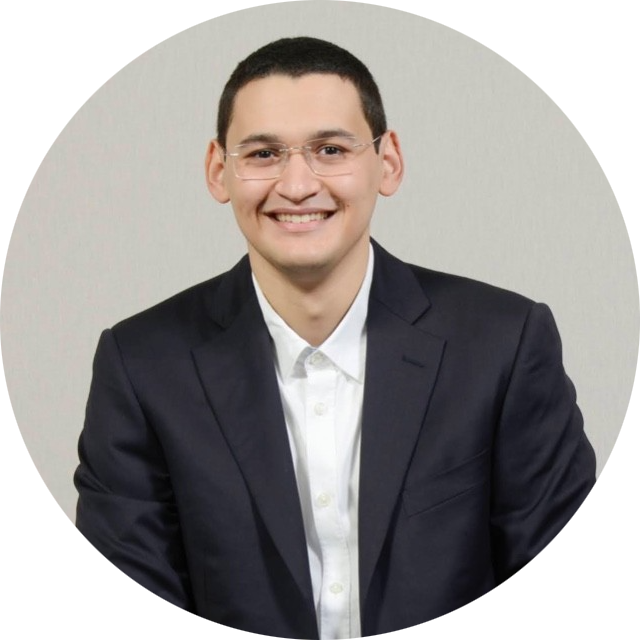
\includegraphics[width=3cm]{images/profilpicture.png}
  \end{minipage}%
  \begin{minipage}[c]{0.8\textwidth}
    \hspace{10pt}
    {\huge \textbf{Zakaria TOZY}} \\ \vspace{10pt}
    \hspace{9pt}
    {\normalsize Analytics Dataginner} \vspace{2pt}
  \end{minipage}
\end{flushleft}

\vspace{-5pt}

\begin{center}
    \small \faPhone\ \texttt{0617407077} \hspace{1pt} $|$
    \hspace{1pt} \faEnvelope\ \texttt{zakaria.tozy@icloud.com} \hspace{1pt} $|$
    \hspace{1pt} \faLinkedin\ \href{https://linkedin.com/in/zakaria-tozy}{\texttt{zakaria-tozy}} \hspace{1pt} $|$
    \hspace{1pt} \faGithub\ \href{https://github.com/zack242}{\texttt{github.com/zack242}} \hspace{1pt} $|$
    \hspace{1pt} \faMapMarker\ Paris
\end{center}

\vspace{10pt}
\section{Résumé}
Ingénieur en Systèmes d'Information et Data Science avec une double formation (ECE Paris/Polytechnique), combinant expertise en ingénierie des données et en analyse. Je recherche un poste en CDI pour mettre à profit mes compétences techniques et analytiques au service de projets à forte valeur ajoutée.

\vspace{10pt}
\section{Compétences}
\textbf{Programmation:} \texttt{Python}, \texttt{SQL}, \texttt{Java}, \texttt{C++}, \texttt{C#} \\
\textbf{Data Engineering:} \texttt{Pandas}, \texttt{NumPy}, \texttt{ETL}, \texttt{Data Pipelines} \\
\textbf{Cloud Databases:} \texttt{BigQuery}, \texttt{Snowflake}, \texttt{GCP}, \texttt{dbt} \\
\textbf{Machine Learning:} \texttt{Scikit-Learn}, \texttt{NLP}, \texttt{LLM} \\
\textbf{Devops:} \texttt{Docker}, \texttt{CI/CD}, \texttt{Git}, \texttt{Scrum} \\
\textbf{Soft Skills:} \texttt{Communication}, \texttt{Esprit d'analyse}, \texttt{Storytelling}, \texttt{Business Acumen} \\
\textbf{Langues:} Français (Bilingue), Arabe (Bilingue), Anglais (Courant - TOEIC 875) \\

\vspace{10pt}
\section{Formation}
\resumeSubHeadingListStart
\resumeSubheading
{Ingénieur en Systèmes d'Information et Big Data Analytics}{Janv 2024}
{École Centrale d'Électronique (ECE Paris)}{}

\resumeSubheading
{Master 2 en Data Sciences}{Janv 2024}
{Institut Polytechnique de Paris (École polytechnique)}{}

\resumeSubHeadingListEnd

\vspace{10pt}
\section{Expérience Professionnelle}
\resumeSubHeadingListStart
\resumeSubheading
{}{}
{AXA Investment Managers - AXA IM}{}

\resumeSubheading
{}{}
{Kalima Blockchain et IoT}{}

\resumeSubheading
{}{}
{Le Crédit Lyonnais - LCL}{}

\resumeSubHeadingListEnd

\vspace{10pt}
\section{Projets}
\resumeItemListStart
\textbf{Bitcoin Analysis} -  \\
\textbf{Twitter Real-time Analysis} -  \\
\textbf{Energy Disaggregation \@Capgemini} -  \\
\resumeItemListEnd


\end{document} 